\documentclass[11pt,preprint, authoryear]{elsarticle}

\usepackage{lmodern}
%%%% My spacing
\usepackage{setspace}
\setstretch{1.2}
\DeclareMathSizes{12}{14}{10}{10}

% Wrap around which gives all figures included the [H] command, or places it "here". This can be tedious to code in Rmarkdown.
\usepackage{float}
\let\origfigure\figure
\let\endorigfigure\endfigure
\renewenvironment{figure}[1][2] {
    \expandafter\origfigure\expandafter[H]
} {
    \endorigfigure
}

\let\origtable\table
\let\endorigtable\endtable
\renewenvironment{table}[1][2] {
    \expandafter\origtable\expandafter[H]
} {
    \endorigtable
}


\usepackage{ifxetex,ifluatex}
\usepackage{fixltx2e} % provides \textsubscript
\ifnum 0\ifxetex 1\fi\ifluatex 1\fi=0 % if pdftex
  \usepackage[T1]{fontenc}
  \usepackage[utf8]{inputenc}
\else % if luatex or xelatex
  \ifxetex
    \usepackage{mathspec}
    \usepackage{xltxtra,xunicode}
  \else
    \usepackage{fontspec}
  \fi
  \defaultfontfeatures{Mapping=tex-text,Scale=MatchLowercase}
  \newcommand{\euro}{€}
\fi

\usepackage{amssymb, amsmath, amsthm, amsfonts}

\def\bibsection{\section*{References}} %%% Make "References" appear before bibliography


\usepackage[round]{natbib}

\usepackage{longtable}
\usepackage[margin=2.3cm,bottom=2cm,top=2.5cm, includefoot]{geometry}
\usepackage{fancyhdr}
\usepackage[bottom, hang, flushmargin]{footmisc}
\usepackage{graphicx}
\numberwithin{equation}{section}
\numberwithin{figure}{section}
\numberwithin{table}{section}
\setlength{\parindent}{0cm}
\setlength{\parskip}{1.3ex plus 0.5ex minus 0.3ex}
\usepackage{textcomp}
\renewcommand{\headrulewidth}{0.2pt}
\renewcommand{\footrulewidth}{0.3pt}

\usepackage{array}
\newcolumntype{x}[1]{>{\centering\arraybackslash\hspace{0pt}}p{#1}}

%%%%  Remove the "preprint submitted to" part. Don't worry about this either, it just looks better without it:
\makeatletter
\def\ps@pprintTitle{%
  \let\@oddhead\@empty
  \let\@evenhead\@empty
  \let\@oddfoot\@empty
  \let\@evenfoot\@oddfoot
}
\makeatother

 \def\tightlist{} % This allows for subbullets!

\usepackage{hyperref}
\hypersetup{breaklinks=true,
            bookmarks=true,
            colorlinks=true,
            citecolor=blue,
            urlcolor=blue,
            linkcolor=blue,
            pdfborder={0 0 0}}


% The following packages allow huxtable to work:
\usepackage{siunitx}
\usepackage{multirow}
\usepackage{hhline}
\usepackage{calc}
\usepackage{tabularx}
\usepackage{booktabs}
\usepackage{caption}


\newenvironment{columns}[1][]{}{}

\newenvironment{column}[1]{\begin{minipage}{#1}\ignorespaces}{%
\end{minipage}
\ifhmode\unskip\fi
\aftergroup\useignorespacesandallpars}

\def\useignorespacesandallpars#1\ignorespaces\fi{%
#1\fi\ignorespacesandallpars}

\makeatletter
\def\ignorespacesandallpars{%
  \@ifnextchar\par
    {\expandafter\ignorespacesandallpars\@gobble}%
    {}%
}
\makeatother

\newenvironment{CSLReferences}[2]{%
}

\urlstyle{same}  % don't use monospace font for urls
\setlength{\parindent}{0pt}
\setlength{\parskip}{6pt plus 2pt minus 1pt}
\setlength{\emergencystretch}{3em}  % prevent overfull lines
\setcounter{secnumdepth}{5}

%%% Use protect on footnotes to avoid problems with footnotes in titles
\let\rmarkdownfootnote\footnote%
\def\footnote{\protect\rmarkdownfootnote}
\IfFileExists{upquote.sty}{\usepackage{upquote}}{}

%%% Include extra packages specified by user

%%% Hard setting column skips for reports - this ensures greater consistency and control over the length settings in the document.
%% page layout
%% paragraphs
\setlength{\baselineskip}{12pt plus 0pt minus 0pt}
\setlength{\parskip}{12pt plus 0pt minus 0pt}
\setlength{\parindent}{0pt plus 0pt minus 0pt}
%% floats
\setlength{\floatsep}{12pt plus 0 pt minus 0pt}
\setlength{\textfloatsep}{20pt plus 0pt minus 0pt}
\setlength{\intextsep}{14pt plus 0pt minus 0pt}
\setlength{\dbltextfloatsep}{20pt plus 0pt minus 0pt}
\setlength{\dblfloatsep}{14pt plus 0pt minus 0pt}
%% maths
\setlength{\abovedisplayskip}{12pt plus 0pt minus 0pt}
\setlength{\belowdisplayskip}{12pt plus 0pt minus 0pt}
%% lists
\setlength{\topsep}{10pt plus 0pt minus 0pt}
\setlength{\partopsep}{3pt plus 0pt minus 0pt}
\setlength{\itemsep}{5pt plus 0pt minus 0pt}
\setlength{\labelsep}{8mm plus 0mm minus 0mm}
\setlength{\parsep}{\the\parskip}
\setlength{\listparindent}{\the\parindent}
%% verbatim
\setlength{\fboxsep}{5pt plus 0pt minus 0pt}



\begin{document}



\begin{frontmatter}  %

\title{Question 3}

% Set to FALSE if wanting to remove title (for submission)




\author[Add1]{Peter Meihuizen}
\ead{21831041@sun.ac.za}





\address[Add1]{Stellenbosch University}



\vspace{1cm}





\vspace{0.5cm}

\end{frontmatter}

\setcounter{footnote}{0}



%________________________
% Header and Footers
%%%%%%%%%%%%%%%%%%%%%%%%%%%%%%%%%
\pagestyle{fancy}
\chead{}
\rhead{}
\lfoot{}
\rfoot{\footnotesize Page \thepage}
\lhead{}
%\rfoot{\footnotesize Page \thepage } % "e.g. Page 2"
\cfoot{}

%\setlength\headheight{30pt}
%%%%%%%%%%%%%%%%%%%%%%%%%%%%%%%%%
%________________________

\headsep 35pt % So that header does not go over title




\hypertarget{introduction}{%
\section{\texorpdfstring{Introduction
\label{Introduction}}{Introduction }}\label{introduction}}

This question shows the popularity of different songs for Metallica and
Coldplay. I will try to analyse these different songs to see what makes
a song popular.

\hypertarget{analysis}{%
\section{\texorpdfstring{Analysis
\label{Analysis}}{Analysis }}\label{analysis}}

I first need to import the data for both Coldplay and Metallica's songs.

So I want to look at what makes songs popular, so I'm going to do some
scatter plots to plot the songs various aspects with their popularity to
see how they compare. To do this I'm going to build a function which
makes a scatterplot.

Plotting the scatterplot shows as follows:

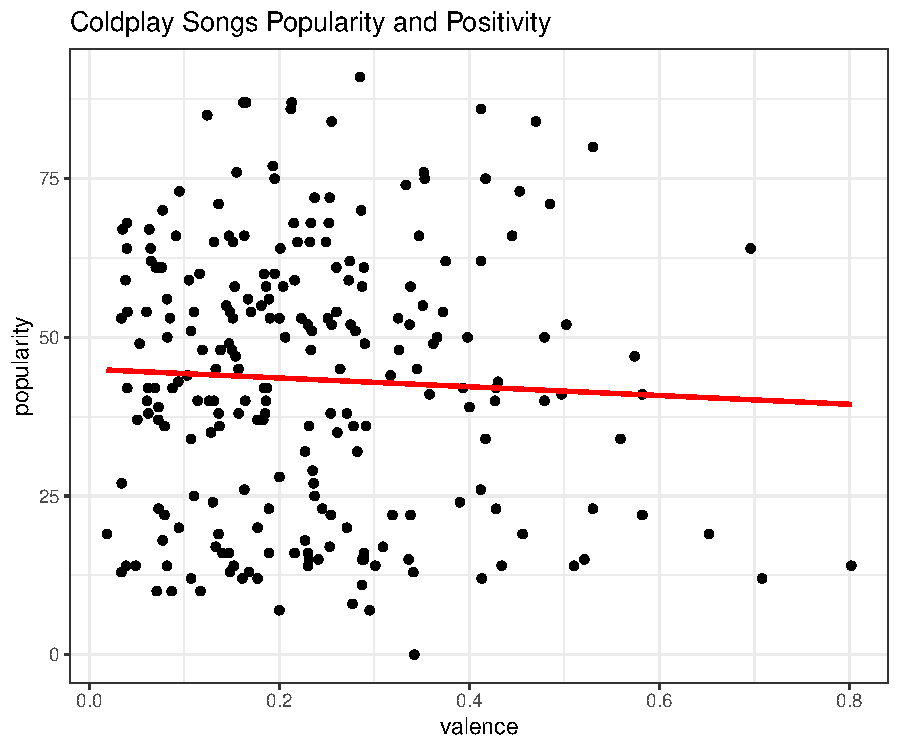
\includegraphics{Question_3_files/figure-latex/unnamed-chunk-2-1.pdf}

It can be seen that Coldplay's music mostly has a lower valence, meaning
it resembles mostly negative emotions, and it appears that there is a
slight negative correlation between vlence and popualrity, suggesting
more positive music does slightly worse than more negative music.

Everyone likes to dance right? So what effect does the danceability have
on the popularity of their songs?

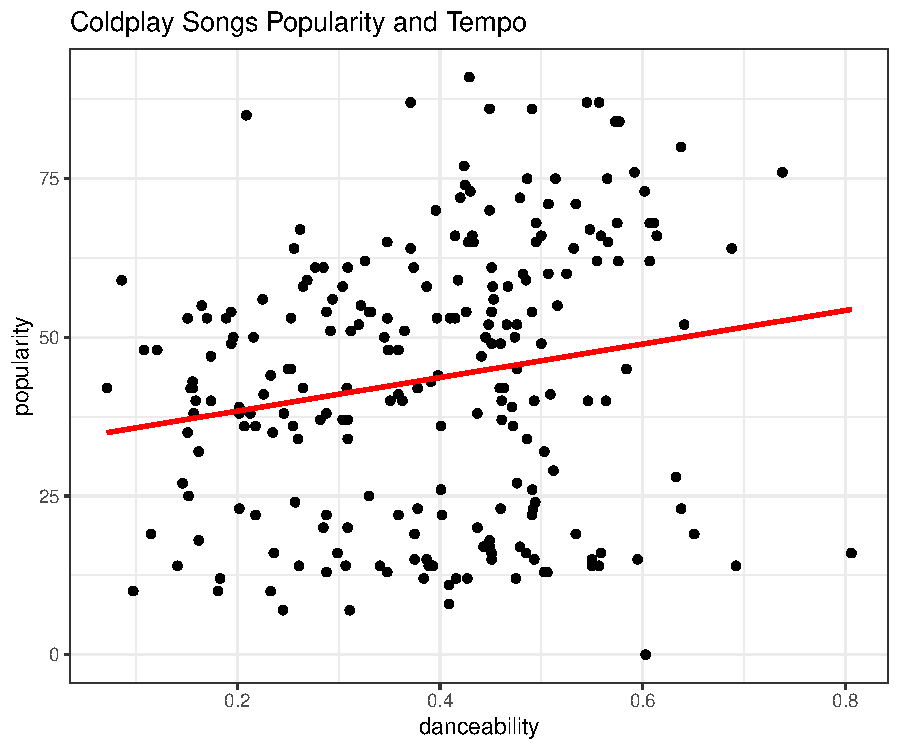
\includegraphics{Question_3_files/figure-latex/unnamed-chunk-3-1.pdf}

Again it appears that danceability has a positive effect on the
popularity of Coldplay's songs.

Ok what about Metallica?

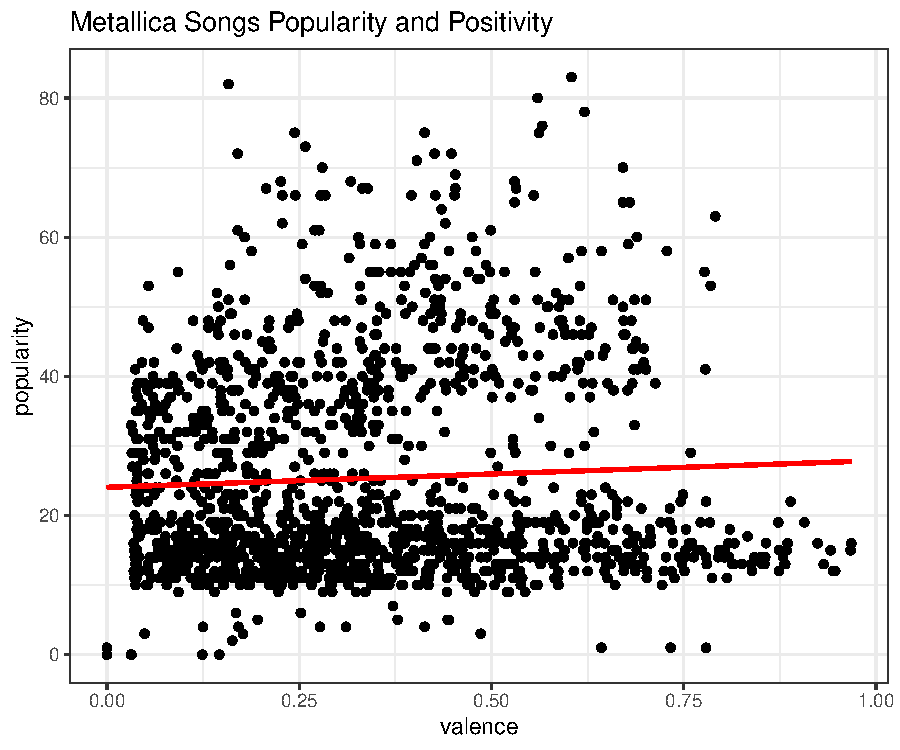
\includegraphics{Question_3_files/figure-latex/unnamed-chunk-4-1.pdf}

There seems to be minimal correlation between valence and popularity for
Metallica's songs. It seems as though their songs are more concentrated
around a low valence, suggesting they express negative emotions. However
their more positive songs are slgihtly more popular as is suggested by
the very gradual slope of the correlation line.

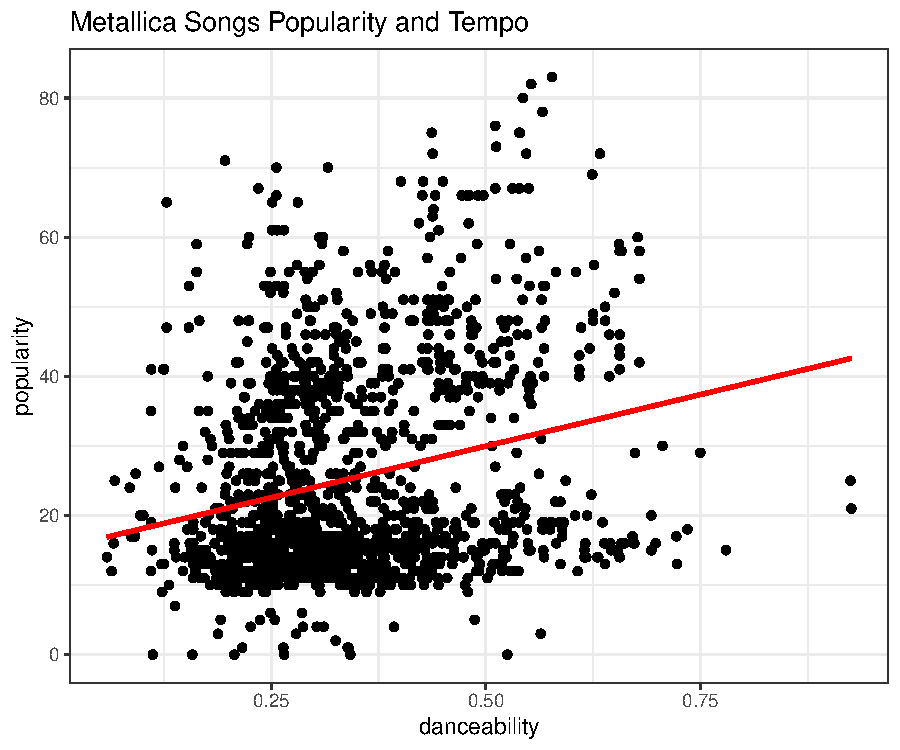
\includegraphics{Question_3_files/figure-latex/unnamed-chunk-5-1.pdf}

Again, the same as was seen with Coldplay, danceability increases the
popularity of Metallica's songs, despite the majority of their songs
being lower on the danceability scale.

Ok so it seems as though danceability makes a particular bands songs
more popular. So let's see how the popularity and danceablility was
distributed across their various albums and see whether these are
linked. In order to do this lets make a function that looks at the
distribution of the danceability of the different albums of Coldplay and
Metallica.

I'm just going to rename the album\_name column in the Coldplay data
frame so that it is the same as in the Metallica data set. I am also
going to get rid of the live albums and songs.

Now ploting the boxplots, first by popularity:

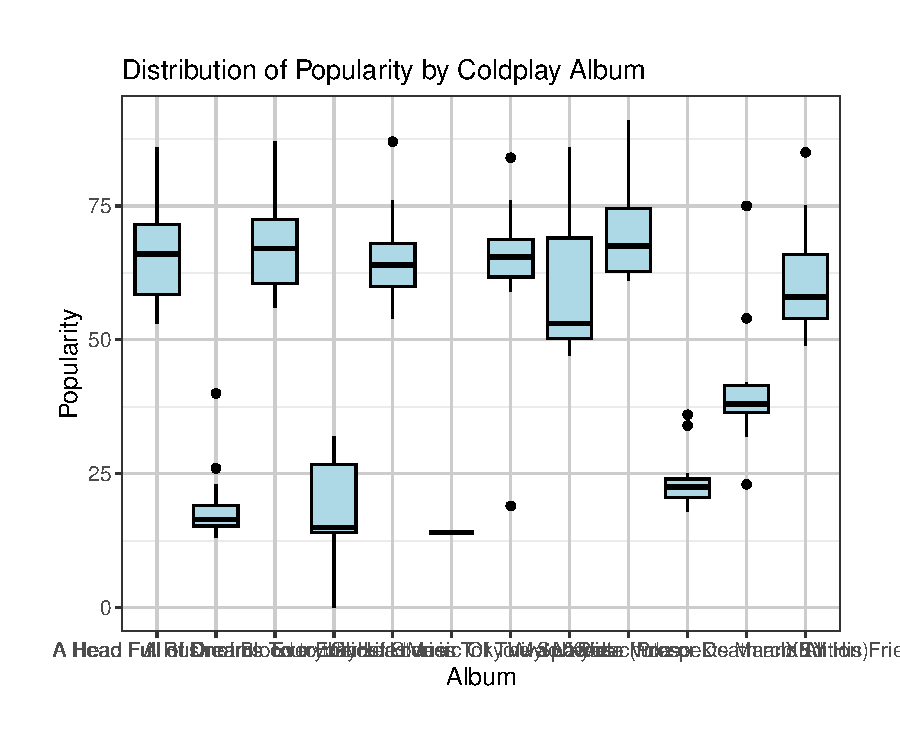
\includegraphics{Question_3_files/figure-latex/unnamed-chunk-7-1.pdf}

So as can be seen Coldplay's albums vary quite a lot in terms of there
popularity, some were significantly more popular than others. What abou
the daceability of their albums?

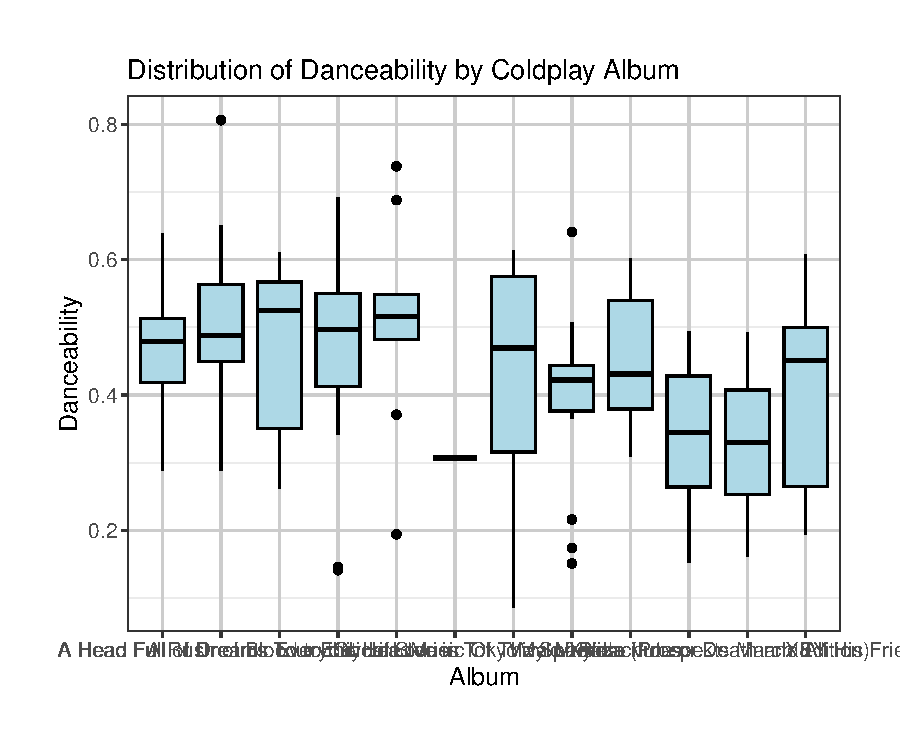
\includegraphics{Question_3_files/figure-latex/unnamed-chunk-8-1.pdf}

It appears as though the distribution of danceable songs on Coldplay's
albums have been pretty similar across albums.

How about Metallica now. First I need to remove the live songs and
albums.

Now to look at the popularity and danceability of the albums. First
popularity.

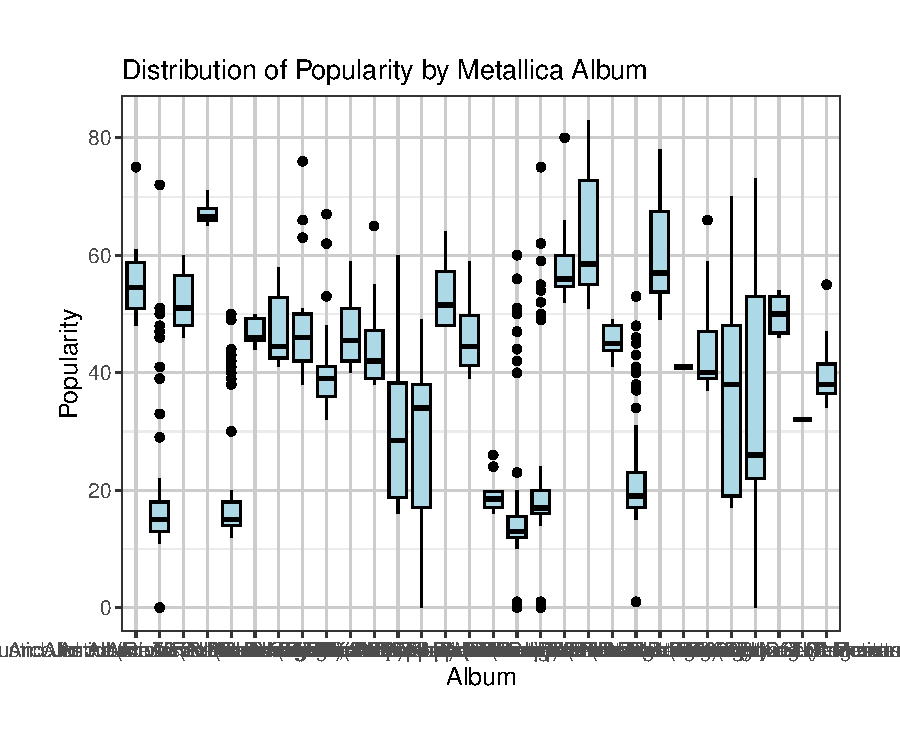
\includegraphics{Question_3_files/figure-latex/unnamed-chunk-10-1.pdf}

Ok similar to Coldplay there are some differences in popularity between
Matallica's albums. Now let's look at their danceability.

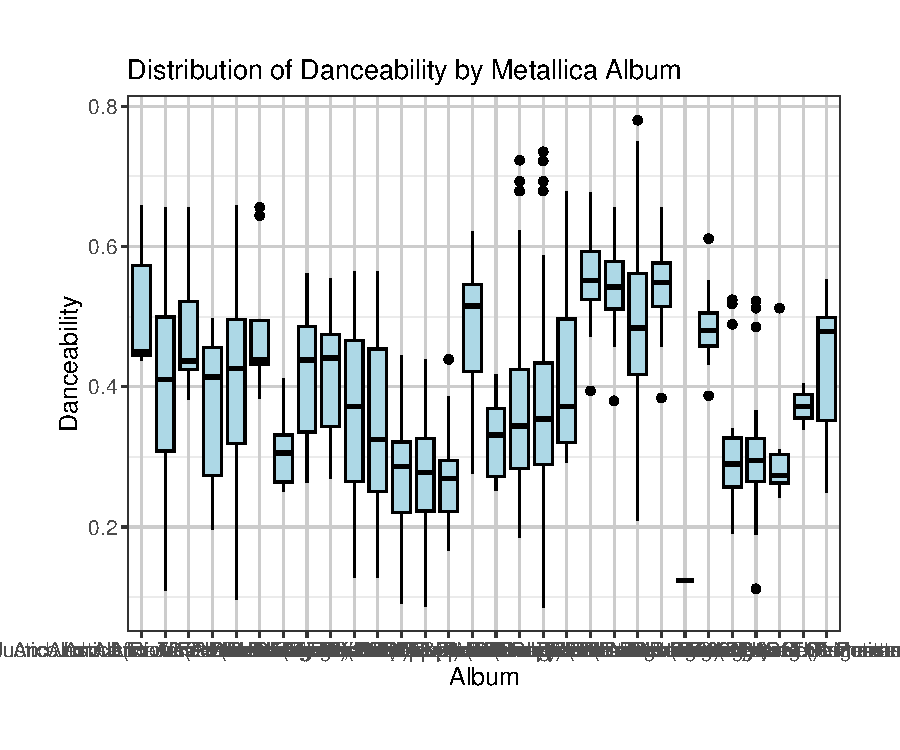
\includegraphics{Question_3_files/figure-latex/unnamed-chunk-11-1.pdf}

As can be seen there's more variation within albums around the
dancability of Metallica's songs, however this variation is seen in most
of there albums suggesting they do not really change their methods
between albums.

\bibliography{Tex/ref}





\end{document}
